\chapter{Medizinische Grundlagen}

\section{Ernährung}

Die Ernährung steht im direkten Zusammenhang mit dem Blutzuckerspiegel und damit mit der Körperhomöostase. Bei der Homöostase wird ein Gleichgewichtszustand eines Systems durch einen sich selbst regelnden Prozess aufrechterhalten. Beispiele für eine Homöostase sind die Regulierung der Körpertemperatur durch Schwitzen oder die Regulierung des Blutzuckerspiegels durch Insulin. 

Der menschliche Stoffwechsel (Metabolismus) kann in eine anabole und katabole Reaktion unterteilt werden. Bei der anabolen Reaktion werden körpereigene Stoffe aus einfachen Bausteinen unter Energieverbrauch \textit{aufgebaut}. Bei der katabolen Reaktion werden zur Energiegewinnung komplexe Nahrungsstoffe zu einfacheren Stoffen abgebaut. 

Der Energiebedarf eines Menschen setzt sich aus seinem Grundumsatz (Alter, Geschlecht, Grösse usw.), seinem Leistungsumsatz (Abhängig von der körperlichen Aktivität) und den Verdauungsverlusten zusammen. Als Energiezufuhr dienen dem Körper folgende Stoffe:
\begin{description}
	\item[Kohlenhydrate (Zucker und Stärken)] \hfil \\
	Dienen zur schnellen Energieversorgung. Abbildung \ref{fig:kohlenhydrate} zeigt die vier Gruppen in die Kohlenhydrate unterteilt sind.
	
	\item[Eiweisse (Proteine)] \hfil \\
	Es sind 20 verschiedenen Aminosäuren bekannt, die 	aneinandergereiht unterschiedlichste Proteine bilden. Die Reihenfolge	der Aminosäuren entscheidet dabei über die biologische Funktion der Proteine.	Proteine haben einen enorm breiten Einsatzbereich. Sie übernehmen mechanische Funktionen (z.B. Fingernägel)	oder agieren als Katalysatoren bei biochemischen Prozessen (Enzyme). Andere Proteine sind wichtig als Signalmolekül (Hormone), bei der Immunreaktion, Gewebebildung usw.
	
	\item[Fette (Lipide)] \hfil \\
	Fette können in sieben Kategorien (Fettsäuren, Wachse usw.) eingeteilt werden und sind meist schwer wasserlöslich. Die biologische Funktion besteht	aus Energieträger, Bildung der Zellmembran und als Botenstoff.
	
	\item[Vitamine] \hfil \\
	Als Vitamine bezeichnet man organische Verbindungen, die für viele lebenswichtige Funktionen benötigt werden, die der Stoffwechsel jedoch nicht bedarfsdeckend erzeugen kann. Somit müssen einige Vitamine mit der Nahrung aufgenommen werden und sind somit essentiell. Unterteilt werden die Vitamine in fettlöslich (lipophile)	und wasserlöslich (hydrophile). Sie kommen in der unbelebten Natur nicht vor und	müssen erst von Pflanzen, Bakterien oder Tieren gebildet werden. Beim Menschen kann man von 13 organischen	Verbindungen sprechen, die als Vitamine gelten (davon sind 11 essentiell).
	
	\item[Mineralstoffe] \hfil \\
	Mineralstoffe sind z.B. für den Knochenbau (Calcium) zuständig.
\end{description}

\begin{figure}
\centering
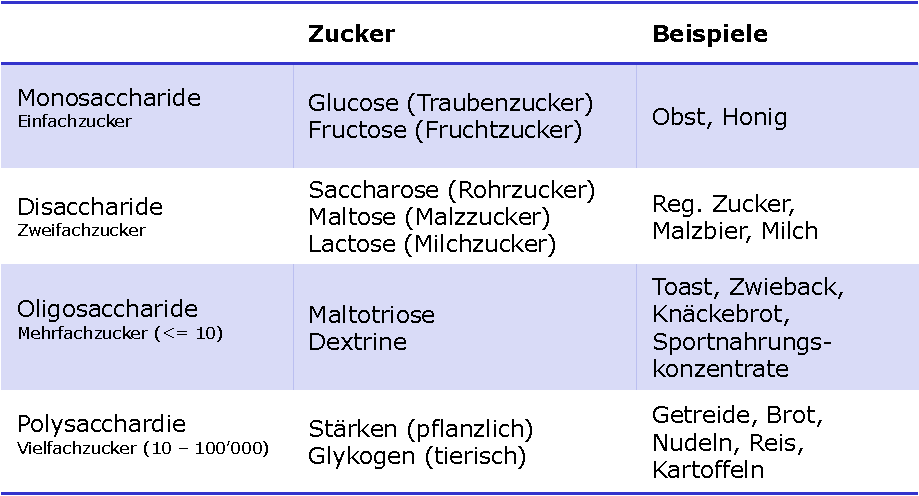
\includegraphics[width=0.7\linewidth]{fig/kohlenhydrate}
\caption{Vier Gruppen von Kohlenhydrate}
\label{fig:kohlenhydrate}
\end{figure}

\section{Verdauung}

TL;DR \href{https://www.youtube.com/watch?v=gcP0AiMDjes}{https://www.youtube.com/watch?v=gcP0AiMDjes}

Der Verdauungsvorgang beginnt bereits in der Mundhöhle mit der Aufnahme und Zerkleinerung der Nahrung. Dort wird die Nahrung in Speisebrei umgewandelt und zuckerspaltende Enzyme beginnen die Verdauung. Im Magen wird der Speisebrei chemisch zerkleinert durch den stark sauren Magensaft (pH 1.5 - 2). Der Magensaft besteht aus Wassser, Schleim, Salzsäure und eiweissspaltenden Enzymen (Pepsin). Nach ca. 1 bis 5 Std. wird der Speisebrei in den Dünndarm weitergeschoben. 

Die Bauchspeicheldrüse produziert ca. 2 l Pankreassaft (Lauge), welche im Zwölffingerdarm ausgeschüttet wird und dort das saure Milieu neutralisiert. Der Pankreassaft enthält zahlreiche Enzyme zur Fett-, Eiweiss- und Kohlenhydratverdauung. Im Inselapparat der Bauchspeicheldrüse werden Hormone zur Regulation des Blutzuckers (Insulin und Glukagon) gebildet. Die Gallenblase gibt zusätzlich Gallensaft in den Zwölffingerdarm ab, damit sich die Fette mit dem wässrigen Mageninhalt vermischen.

Im Dünndarm findet die eigentliche Verdauung und Aufnahme (Resorbtion) statt. Durch die Enzyme der Bauchspeicheldrüse werden die Nährstoffe in resorbierbare Bestandteile gespalten. Die starke Muskulatur um den Dünndarm ermöglicht eine gute Durchmischung des Darminhaltes. Zur Steigerung der Resorption ist die Oberfläche der Schleimhaut durch Falten, Zotten und Mikrovilli stark vergrössert. Die Nährstoffe (Aminosäuren, Fettsäuren und Zucker) werden über das Kapillarnetz aufgenommen und der Leber zugeführt.

Die Leber ist mit rund 1.5 bis 2 kg die grösste Drüse des Menschen. Pro Minute fliessen 1.5 l arterielles Blut durch das Organ. Als Stoffwechselorgan übernimmt sie wichtige Funktionen des Kohlenhydrat-, Eiweiss- und Fettstoffwechsels sowie der Entgiftung. Die Gallensäure der Gallenflüssigkeit emulgiert im Darm Fette und ermöglicht dadurch die Resorption. Die im Darm resorbierten Nährstoffe gelangen über die Pfortader in die Leber. Kohlenhydrate als Glykogen werden gespeichert und bei Bedarf wieder abgegeben. 

Im Dickdarm findet die Rückresoprption von Wasser und Salzen statt. Unverdaute Nahrungsreste werden durch Bakterien via Gärung und Fäulnisprozesse zersetzt. Die Schleimhaut hat eine viel geringere Oberflächenvergrösserung als die des Dünndarms. Abbildung \ref{fig:verdauung} zeigt einen Gesamtüberblick über diese Organe.

\begin{figure}
\centering
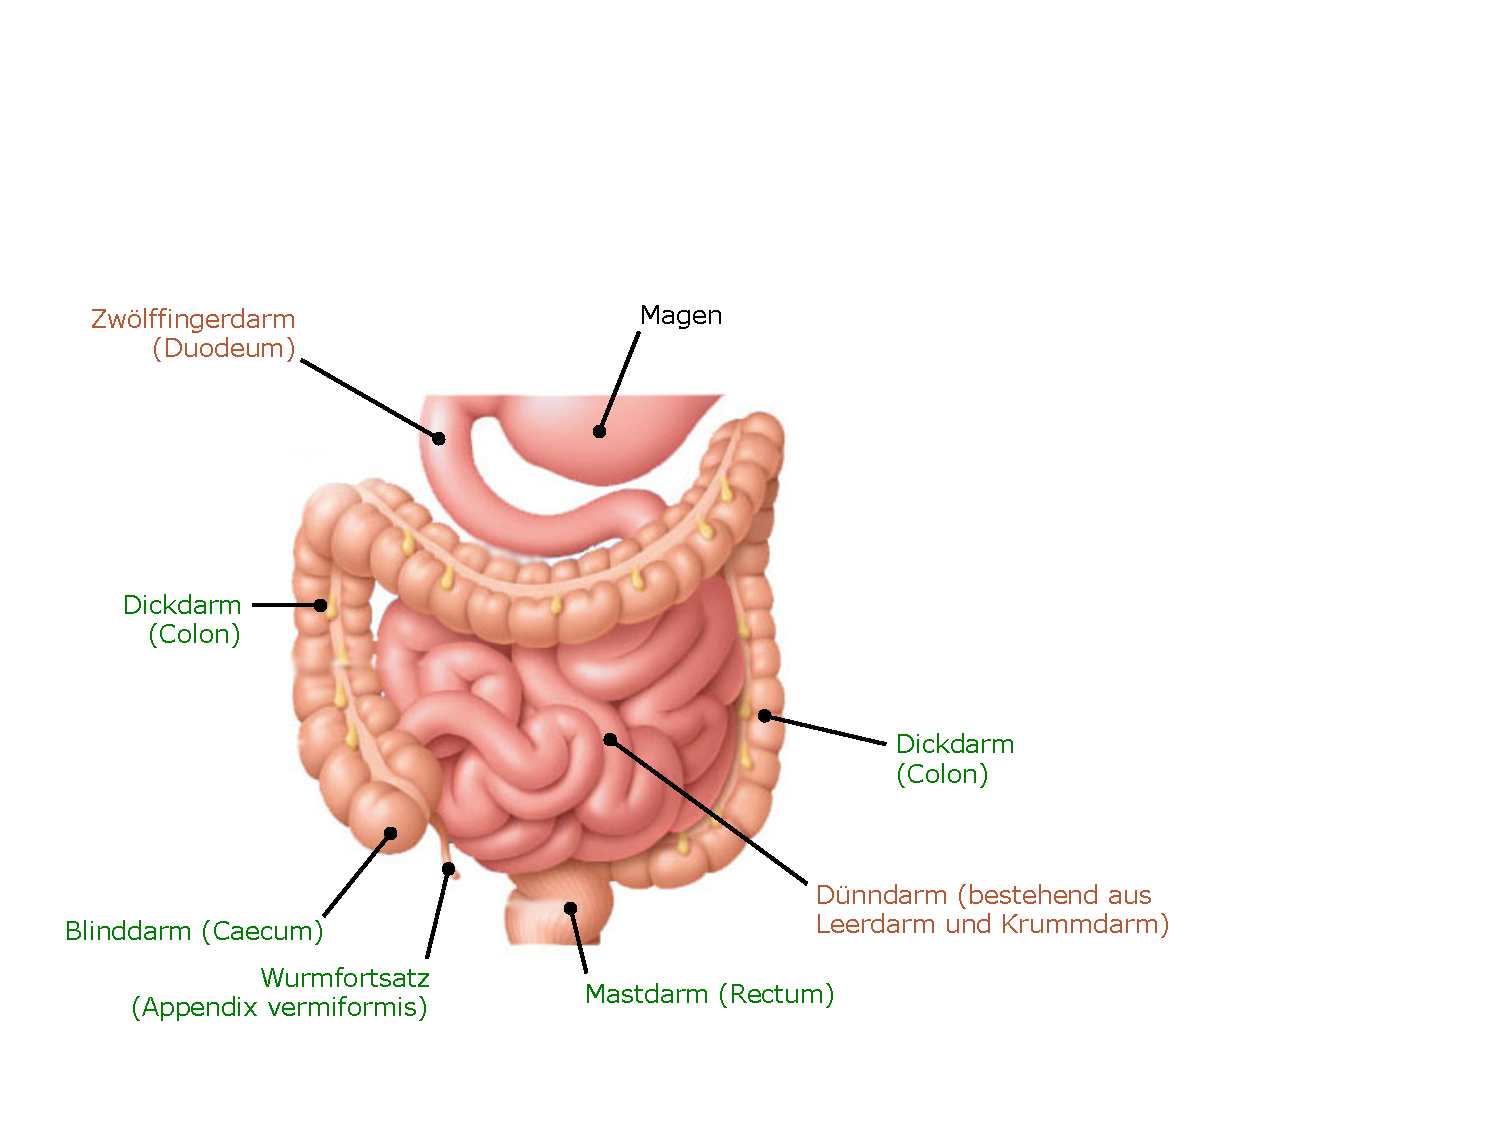
\includegraphics[width=0.7\linewidth]{fig/verdauung}
\caption{Übersicht Verdauung}
\label{fig:verdauung}
\end{figure}

\newpage

Nachfolgend werden die verschiedenen Verdauungsvorgänge stichwortartig beschrieben:
\begin{description}
	\item[Kohlenhydratverdauung] \hfil  \\
	In der Mundhöhle verkleinern die Amylasen die Kohlenhydrate. Im Zwölffingerdarm werden sie durch die Pankreasamylase weiter verkleinert. Im Dünndarm werden sie durch zuckerspaltende Enzyme der Dünndarmschleimhaut zu Monosacchariden (Glukose, Galaktose, Fruktose) aufgespalten. Diese werden dann durch aktiven oder passiven Transport aufgenommen und über die Leber in den Blutkreislauf weitergeleitet.
	
	\item[Proteinverdauung] \hfil \\
	Die Eiweisse werden im Magen durch Pepsine in Bruchstücke (Peptide) zerkleinert. Der Abbau geht im Zwölffingerdarm weiter. Im Dünndarm werden sie aktiv aufgenommen und passiv in die Blutbahn abgegeben.
	
	\item[Fettverdauung] \hfil \\
	Das Fett wird durch die Gallensäure im Zwölffingerdarm emulgiert (aufgelöst) und durch Lipase der Pankreas gespalten. Diese werden dann im Dünndarm aufgenommen.
\end{description}
\textit{Endozytose} beschreibt die Aufnahme von Substanzen ind die Zelle hinein. Exozytose entfernt die Abfall- und Nebenprodukte aus den Stoffwechselvorgängen regelmässig aus den Zellen. Die in die Zellen verteilten Energieträger (Kohlenhydrate, Proteine und Fette) werden dort oxidiert. Die dabei entstehende Energie wird in energiereichen Bindungen in einem Molekül namens \textbf{Adenosintriphosphat}, oder ATP gespeichert. ATP wird aus \textbf{Adenosindiphosphat} (ADP) gebildet, indem eine Phosphatgruppe mit einer energiereichen Bindung geknüpft wird. Mitochondrien werden dadurch als die \textit{Kraftwerke} der Zellen bezeichnet, weil in ihnen das energiereiche Molekül ATP gebildet wird.

\newpage

\section{Blut}

Blut ist Gewebe mit einer Temperatur von 38$^\circ$C, welches abhängig von der Sauerstoffsättigung seine Farbe ändert (hoher Sauerstoffgehalt -- hellrote Farbe). Das Blutvolumen beträgt 8\% der Körpermasse (5 – 6l Mann, 4 –
5l Frau). Das Blut hat folgende Funktionen:
\begin{description}
	\item[Transport] Wärmeregulation, Stoffverteilung (Nährstoffe und Abfall), Gasaustausch, Informationsaustausch
	\item[Regulation / Homöostase] Wasser- und Elektrolythaushalt, pH-Wert
	\item[Schutz / Abwehrfunktion] unspezifische und spezifische Abwehr durch spezielle Blutzellen und Blutgerinnung
\end{description}
Blut besteht aus Blutplasma, weissen Blutkörperchen (bis 10'000 Zellen), roten Blutkörperchen (bis 5 Mio. Zellen) und Blutplättchen (bis 400'000 Zellen). Blutplasma ist der flüssige Anteil des Blutes und der Rest sind die festen Blutzellen.

\subsection{Plasma}

Plasma besteht zu 91\% aus Wasser, 8\% Eiweißstoffe und 1\% aus Salzen sowie anderen Substanzen. Plasmaproteine werden hauptsächlich durch die Leberzellen gebildet und bestehen meist aus \textbf{Albumine} (54\% der Plasmaproteine), \textbf{Globuline} (38\%) und \textbf{Fibrinogene} (7\%). Sie dienen als Antikörper, transportieren Stoffe (z.B. Hormone), sind verantwortlich für die Blutgerinnung und zur Aufrechterhaltung des pH-Werts. Die meisten Stoffe passieren auch die Kapillar- und Zellwände zur Versorgung der Zellen mit Nährstoffen. Anschliessend wird die meiste Flüssigkeit von den Kapillaren wieder aufgenommen (einschliesslich der Stoffwechselabbauprodukte der Zellen). Ein Teil der Flüssigkeit gelangt in die Lymphbahnen.

\subsection{Rote Blutkörperchen (Erythrozyten)}

Erythrozyten werden im roten Knochenmark, aus kernhaltigen Stammzellen gebildet. Enthalten im Inneren Hämoglobin (eisenhaltig) zum Transport des Sauerstoffs/Kohlendioxid (33\% der Zellmasse). Ihre Zellmembran ist stark und elastisch. Sie besitzen keinen Zellkern (Verlust des Kerns bei der Ausreifung) und auch kaum Organellen (\textit{Orgänchen}), was eine Zellteilung verunmöglicht. Die Lebensdauer beträgt ca.120 Tage danach platzen sie. Sie werden durch Makrophagen in der Milz entsorgt. Das Eisen wird rezykliert und der Rest in Bilirubin umgewandelt. Weiterer Abbau in ein braunes Pigment und Ausscheidung im Stuhl. Die Blutgruppe wird hauptsächlich von den Erythrozyten bestimmt. Abbildung \ref{fig:blutgruppen} zeigt einen Überblick über die Antigene/Antikörper.

\begin{figure}
\centering
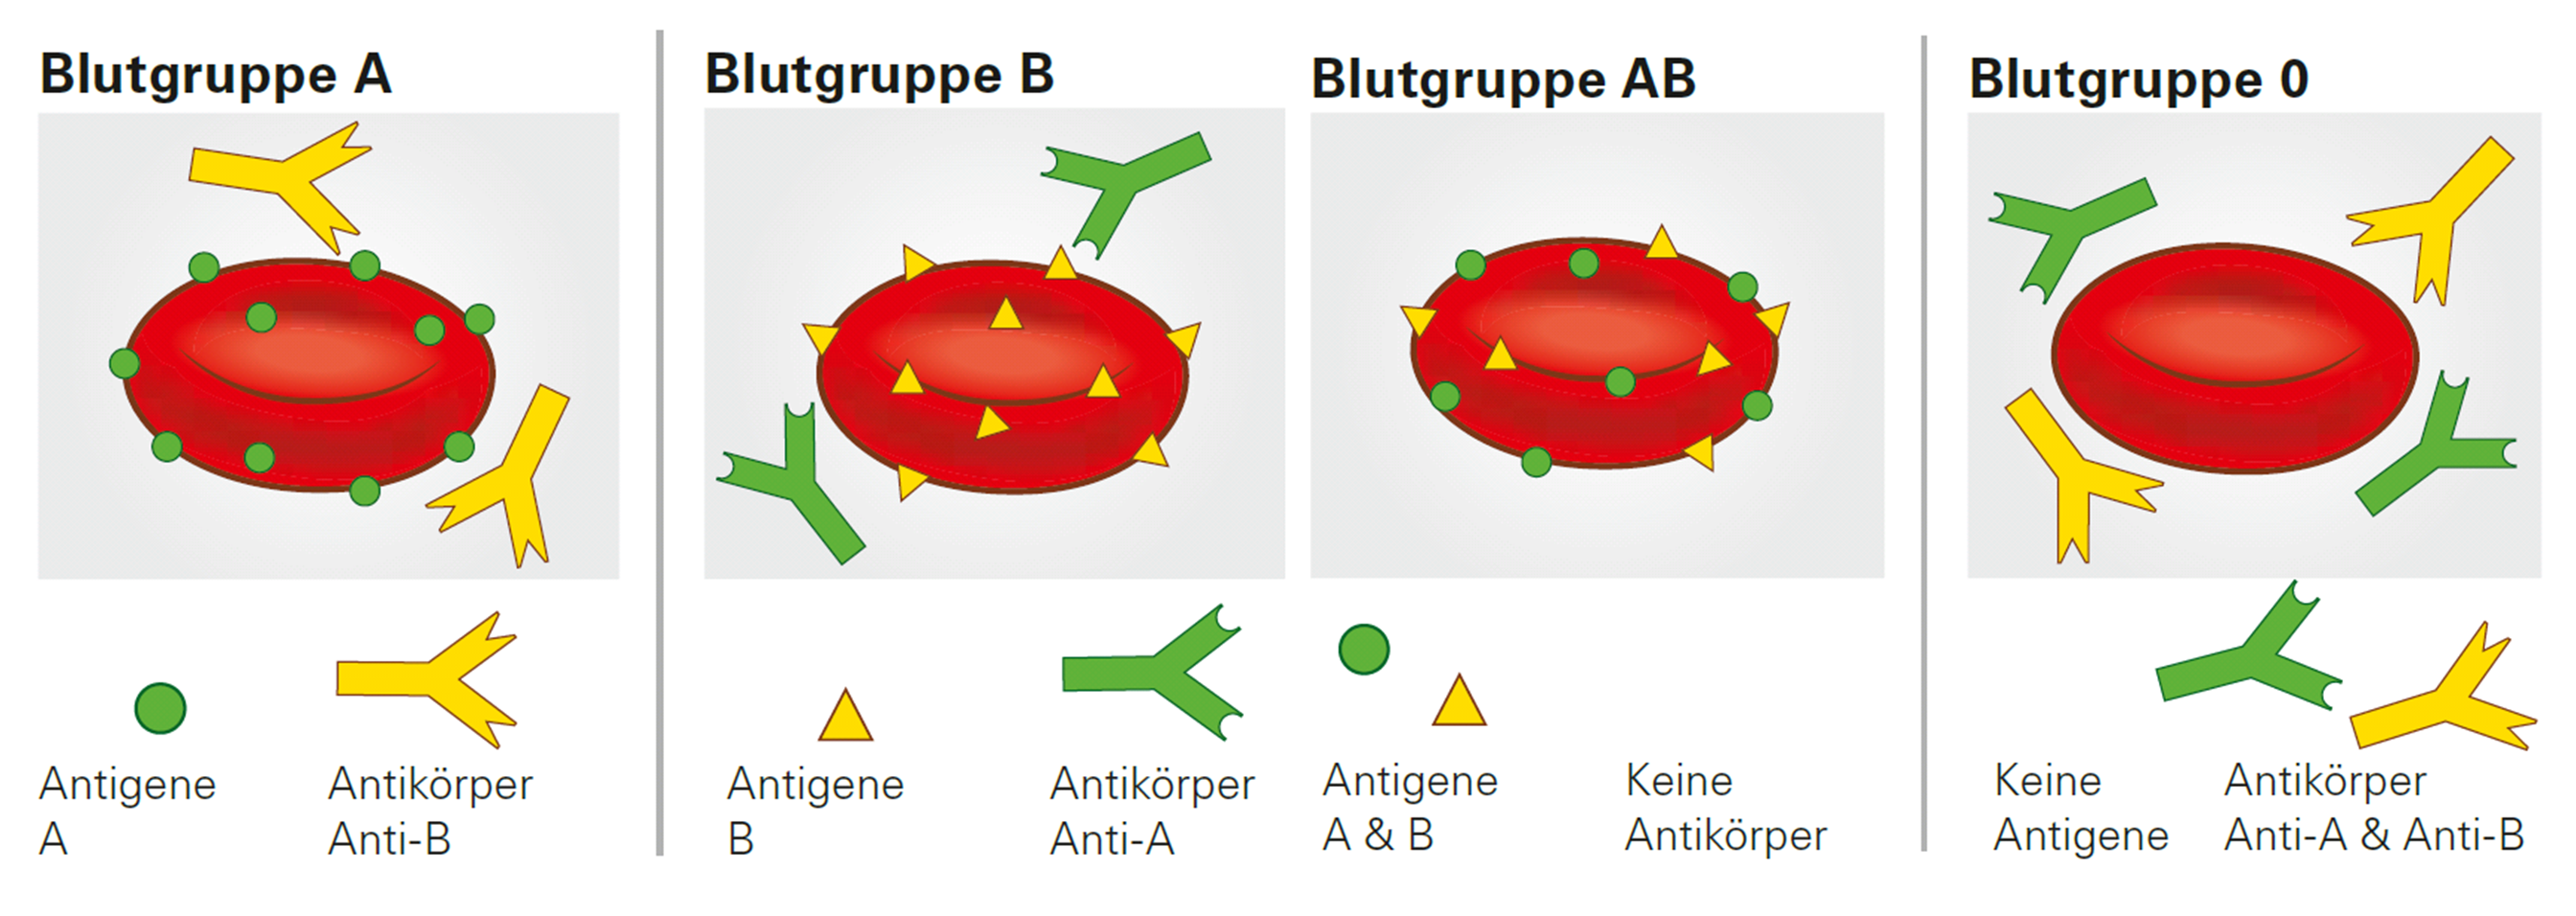
\includegraphics[width=0.7\linewidth]{fig/blutgruppen}
\caption{Blutgruppen}
\label{fig:blutgruppen}
\end{figure}

\subsection{Weisse Blutkörperchen (Leukozyten)}

Leukozyten werden aus Knochenmarktstammzellen erzeugt und können dann zu spezifischen Zellen ausgebildet werden. Eine Stammzelle kann z.B. zu einer T-Zelle werden um Viren, Krebszellen oder transplantierte Zellen zu attackieren. Die erste Schutzfrint gegen Erreger bilden die Haut, Schleimhäute usw. Erst wenn Erreger diese erste Schutzfront durchbrochen haben, kümmert sich das Immunsystem als zweite Schutzfront um sie. Grob wird das Immunsystem in eine spezifische und unspezifische Immunabwehr eingeteilt. Diese beiden Typen werden dann nochmals in eine zelluläre und humorale Abwehr unterteilt. Die zelluläre Abwehr sind feste Zellen (z.B. Leukozyten) wohingegen die humorale Abwehr flüssig ist (z.B. Blutplasma). Die unspezifische Immunabwehr ist bereits von Geburt an vorhanden und besitzt kein Gedächtnis. Dringt ein unbekannter Erreger in den Körper ein wird er von der unspezifischen Immunabwehr unschädlich gemacht und die Antigene des Erregers an die spezifische Immunabwehr übertragen. Antigene sind Andockstellen auf der Oberfläche eines Erregers, anhand dessen die spezifische Immunabwehr die Erreger wieder erkennt und entsprechend reagieren kann.

\subsection{Blutplättchen (Thrombozyten)}

Die Thrombozyten werden im roten Knochenmark gebildet und besitzen wie die Erythrozyten keinen Zellkern. Ihre wichtigste Funktion ist die Blutstillung und Blutgerinnung, indem sie ein Blutgerinsel (Thrombus) bilden. Tritt eine Verletzung einer Blutbahn auf, ziehen sich die Gefässe zusammen (Vasokonstriktion). An der verletzten Stelle lagern sich Thrombozyten ab, welche die Wunde vorerst verschliessen (Blutstillung oder Hämostase). Durch die Freisetzung von Thrombin wird Fibrinogen in Fibrin umgewandelt und bildet ein Netz aus dünnen Faser (Throbmus), welche die Wunde endgültig verkleben. 

\section{Herz}

Das Herz ist ein muskuläres Hohlorgan, das mit rhythmischen Kontraktionen Blut durch den Körper pumpt. Die Grösse entspricht rund 1.5 x der geballte Faust und wiegt ca. 300–350g. Arbeitet nach dem Verdrängungspumpen-Prinzip indem Blut aus den Blutgefässen angesaugt und durch andere Blutgefässe ausgestossen wird. Ein isoliertes Herz vermag bei ausreichender Nährstoffzufuhr über längere Zeit autonom zu schlagen. Herzfrequenz, Erregungsleitungsgeschwindigkeit und Kontraktionskraft werden durch das vegetative Nervensystem gesteuert. Der menschliche Kreislauf besteht aus dem kleineren Lungenkreislauf und dem grösseren Herzkreislauf. Die Wand grösserer Blutgefäße besteht aus drei verschiedenen Schichten:
\begin{itemize}
	\item Innere Schicht (Gefässendothel, \textit{Intima})
	\item Mittlere Schicht (Tunica media, \textit{Media}) mit glatter Muskulatur und elastischen Fasern
	\item Äussere Schicht (Tunica adventitia, \textit{Adventitia}) steht in Verbindung mit dem umliegenden Gewebe.
\end{itemize}
Die elastische Membran findet man nur bei Arterien. Die Muskelschicht der Arterien dienen zur Gefässmotorik (Vasodilatation und Vasokonstriktion). Elastische Eigenschaften herznaher Arterien dämpfen den stark pulsierenden Blutstrom. Venen sind weitlumiger und dünnwandiger als Arterien. Die meisten Venen besitzen Venenklappen, die wie Ventile den Blutstrom zum Herzen lenken und ein Zurückfliessen verhindern. Abbildung \ref{fig:venen} zeigt dieses Prinzip.

\begin{figure}
\centering
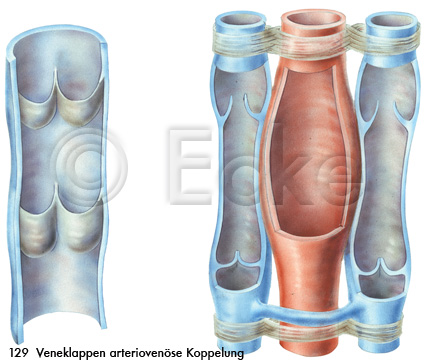
\includegraphics[width=0.4\linewidth]{fig/venen}
\caption{Venenklappen}
\label{fig:venen}
\end{figure}

\section{Endokrinologie}

Endokrine Systeme produzieren Signal- oder Botenstoffe (Hormone) und entlassen diese in die Zirkulation.  Im Gegensatz zum neuronalen System ist die Kommunikation \textit{drahtlos}. Ein bekanntes Hormon ist Insulin. Insulin ist ein Peptid, das aus 51 Aminosäuren besteht. Es wird in den Langenhanschen Inseln der Bauchspeicheldrüse produziert. Die Struktur von Insulin variiert leicht zwischen Säugetieren (Schweineinsulin hat schlechtere Wirkungseffekte als humanes Insulin). Insulin war das erste Protein deren Aminosäuresequenz analysiert wurde und als erstes synthetisiert wurde.

Der Blutzuckerspiegel ist ständigen Schwankungen unterworfen (Sollwert 100 mg Glucose auf 100 ml Blut). Abbildung \ref{fig:blutzucker} zeigt wie der Blutzuckerspiegels mithilfe der Bauchspeicheldrüse und des Hypothalamus (Teil des Zwischenhirns) geregelt wird.

\begin{figure}
\centering
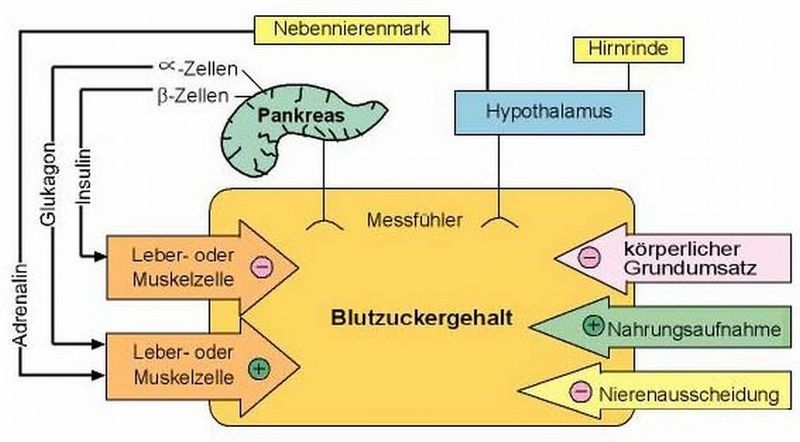
\includegraphics[width=0.7\linewidth]{fig/blutzucker}
\caption{Blutzuckerregelsystem}
\label{fig:blutzucker}
\end{figure}

Bei einer Überzuckerung (Hyperglykämie) zeigt der Blutzuckerspiegel steigt immer weiter an (nach Kohlenhydratreicher Nahrung bis zu 160mg/dl). Als Reaktion darauf schütten Beta-Zellen der Bauchspeicheldrüse Insulin aus. Dadurch gelangt Blutzucker durch die Zellwände in die Zellen wo er verbraucht und/oder als Stärke (= Glykogen) gespeichert wird. 

Bei einer Unterzuckerung (Hypoglykämie) schütten die Alpha-Zellen der Bauchspeicheldrüse Glukagon aus. Dadurch wird in der Leber Glykogen zu Glucose abgebaut und ins Blut abgebeben. Eine Unterzuckerung führt oft zu einer verminderten Hirnleistung, Krampfanfällen, eine vermehrte Adrenalinausschüttung und zittrigen Händen sowie Schweißausbrüchen. In schlimmen Fällen kann es zu einem Schock führen.

Man unterscheidet zwei Formen des Diabetes mellitus (>126 mg/dl): Beim Typ 1 Diabetes produziert der Körper kein Insulin (Autoimmunerkrankung) und beim Typ 2 Diabetes ist die Wirkung des Insulins unzureichend (Insulinresistenz).

\subsection{Typ 1: Jugenddiabetes}

Hauptsächlich Kinder und Jugendliche (3 von 1'000 Kinder) erkranken an dieser Form. Dabei zerstört das Immunsystem die insulinproduzierenden Zellen in der Bauchspeicheldrüse. Typ-1-Diabetiker benötigen mehrmals täglich Insulin. Anzeichen von Typ 1 Diabetes können sein: Ständiger Durst, häufiges Wasser lassen, allgemein schwach fühlen und Gewichtsverlust, Sehstörungen, Juckreiz und Infektionen der Haut oder der Harnwege.

\subsection{Typ 2: Altersdiabetes}

Vornehmlich Menschen in höherem Lebensalter erkranken an Typ 2 Diabetes (häufigste Form von Diabetes, ca. 80 bis 90\% aller Diabetiker). Immer häufiger sind auch jüngere Erwachsene davon betroffen. Übergewicht und ein Mangel an körperlicher Bewegung begünstigen die Erkrankung. Anzeichen von Typ 2 Diabetes können sein: Leichte, aber ständige Müdigkeit und allgemeiner Schwäche, Erkrankung oft durch die Untersuchung anderer Krankheiten wie Herzprobleme, Sehstörungen, Gefühllosigkeit in den Füssen oder schlecht heilende, offene Hautstellen an den Füssen festgestellt.

\subsection{Blutzuckerspiegelmessung}

Es gibt drei Möglichkeiten den Blutzuckerspiegel zu messen.

\subsubsection{Optische Messung}

Eine chemische Reaktion löst eine Farbänderung des Testfeldes aus. Die Farbänderung wird vom Messgerät erfasst und aus der Dauer und Stärke der Änderung der Blutzuckerwert bestimmt.

\subsubsection{Amperometrische Messung}

Das Blut kommt in Kontakt mit Glucose-Oxidase und verschiedener Elektroden. Über eine definierte elektrische Spannung an den Elektroden wird der Strom gemessen (der Strom ist proportional zur Glukosekonzentration der Flüssigkeit). Anhand dieses bestimmt das Gerät den Blutzuckerwert.

\subsubsection{Nichtinvasive Messung}

\begin{itemize}
	\item Optische Spektralanalyse des Augenhintergrundes
	\item Implantierte Mikrospektrometer via spektroskopische Messung des Blutzuckers im nahen Infrarot-Bereich (NIR).
	\item Mit Laser im mittleren Infrarot-Bereich (MIR) kann durch die Haut der Blutzuckerwert bestimmt werden.
	\item Nanopartikel (als Tattoos injiziert) beginnen bei erhöhten Blutzuckerwerten zu fluoreszieren.
	\item Mittels Interferometrie kann der Glukosegehalt des Speichels bestimmt werden.
	\item Glucosebestimmung im Urin (Methode gilt als überholt) ist nur dann möglich, wenn die Glucosekonzentration stark erhöht ist und einen bestimmten Wert überschritten hat.
\end{itemize}